\subsection{Kartesische Produkte von Graphen}
In diesem Teil zeigen wir, was im Bezug auf die Anzahl der Spannbäume geschieht, wenn man das kartesische Produkt von Graphen bildet.\\
Das kartesische Produkt $\,G_1\times G_2\,$ zweier Graphen $\,G1=(V_1,E_1)\,$ und $\,G2=(V_2,E_2)\,$ bezeichnet dabei den Graphen mit Knotenmenge $\,V_1\times V_2\,$ und Kantenmenge $\,(E_1\times V_2)\cup(V_1\times E_2)$,\; wobei zwei Knoten $\,(u_1,u_2), (v_1,v_2) \in (V_1\times V_2)\,$ genau dann in $\,G_1\times G_2\,$ benachbart sind, wenn entweder $\,u_1=v_1\,$ in $\,G_1\,$ oder $\,u_2=v_2\,$ in $\,G_2\,$ ist.\\
\todo[inline, color=yellow]{Ich werde wahrscheinlich ein/zwei Beispiele davon zeigen, z.B. Lattice-Graph, aber nicht mehr, weil das im Grund genommen einfach nur Rechnungen sind und das Matrix-Tree-Theorem nicht mehr als solches angewendet wird, sondern nur über den Satz unten(passt das?)---Antwort:JA->warmup-kapitel}
\todo[inline, color=yellow]{Vielleicht ist es sinnvoll ein weiteres Kapitel mit einfachen Graphen wie Kreis-Graphen, Pfad-Graphen,etc. zu machen, dann könnte man sich in diesem Kapitel fast alle Rechnungen  ersparen und nur ein/zwei Beispiele geben, was man daraus "basteln" kann (Gute Idee?)---Antwort:JA}
\begin{Tms}
 Sei $\,G\,$ ein Graph mit $\,m\,$ Knoten und Eigenwerten $\,\mu_1(G),..,\mu_m(G)\,$ und $\,H\,$ ein Graph mit $\,n\,$ Knoten und Eigenwerten $\,\mu_1(H),..,\mu_n(H)$.\;  \\
Dann hat der Graph $\,G \times H\,$ genau
\begin{equation}
\frac{1}{nm}\displaystyle\prod_{i,j}(\mu_i(G)+\mu_j(H))1_{\{\mu_i(G)+\mu_j(H)\neq0\}}
\end{equation}
Spannbäume.
\label{tmcpG}
\end{Tms}
\textbf{Beweis:}\\
Für diesen Beweis werden wir die Gestalt der Laplacematrix von $\,G \times H\,$ ausnutzen und dann mit Hilfe der linearen Algebra Aussagen über die Eigenwerte treffen.\\
Wir beobachten, dass die Laplacematrix von $\,G\times H\,$ die Kroneckersumme der Laplacematrizen von $\,G\,$ und $\,H\,$ ist.\\
Aus der linearen Algebra wissen wir nun, dass die Eigenwerte der Kroneckersumme $\,L(G) \oplus L(H)\,$ genau $\,\mu_i(G)+\mu_j(H)\,$ mit $\,i \in \{ 1,..,m\}\,$ und$\, j \in \{ 1,..,n\}\,$ sind.\\
Mit Kirchhoffs Matrix-Tree-Theorem folgt nun
\begin{equation}
 \mathit{k}(G \times H) = \frac{1}{nm}\displaystyle\prod_{i,j}(\mu_i(G)+\mu_j(H))1_{\{\mu_i(G)+\mu_j(H)\neq0\}}
\end{equation}
Damit ist unser Satz bewiesen.
\begin{flushright} $\,\Box\,$ \end{flushright} 
\todo[inline]{Beweis ganz sauber fertigmachen, evtl. Quelle in der man was über ide Kroneckersumme nachlesen kann}
Dieses Hilfsmittel erleichtert uns das Berechnen der Anzahl von Spannbäumen kartesischer Produkte von Graphen erheblich. Um das zu demonstrieren, werden wir uns nun drei verschiedene Klassen davon als Beispiele ansehen.

\begin{Bsps}[Zylinder-Graph]
\end{Bsps}
Als erstes, sehr anschauliches Beispiel betrachten wir Zylinder-Graphen $\,C_{m,n}$;
diese sind das kartesische Produkt eines Pfad-Graphen $\,P_m\,$ mit einem Kreisgraphen $\,C_n$.\; \\
In der Abbildung \ref{c8xp3} sehen wir den Zylinder-Graphen $\,C_{3,8}$.\; 
\begin{figure}[H]
  \centering
 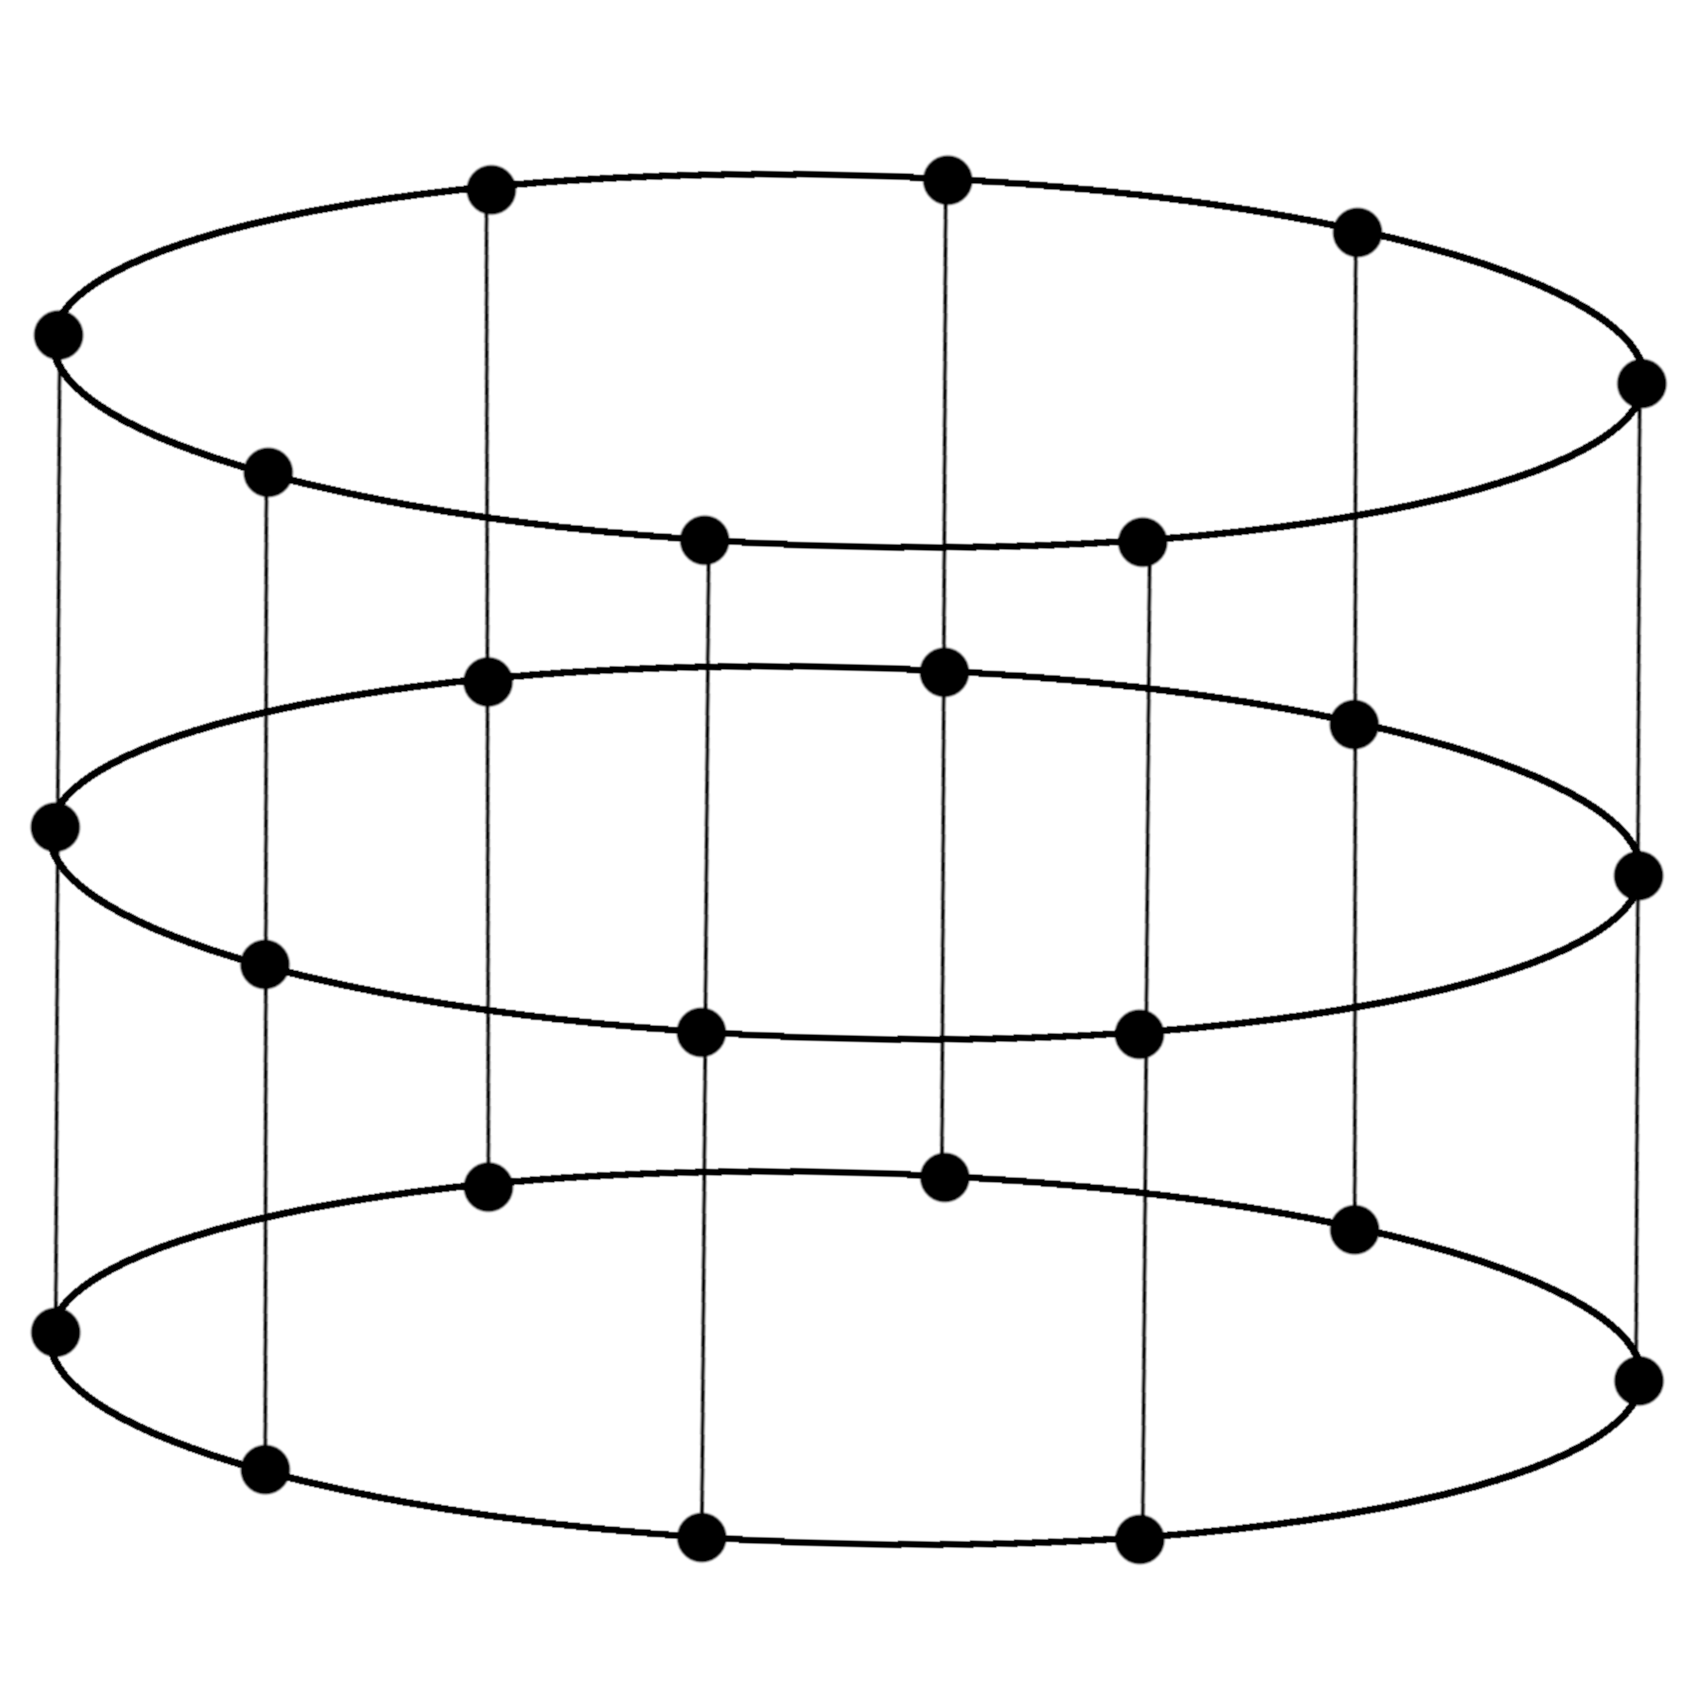
\includegraphics[width=0.25\textwidth]{c8xp3.png}
 \caption{$C_{3,8}$}
 \label{c8xp3} %caption vor label unbedingt
\end{figure}
\begin{Bsps}[Torus-Graph]
%kreis und Kreis
\end{Bsps}
Unser zweites Beispiel sind kartesische Produkte zweier Kreis-Graphen $\,C_m,C_n$.\; \\
Man nennt diese dann auch Torus-Graphen, kurz $\,T_{m,n}$.\;  Hier sehen wir so einen Graphen:
\begin{figure}[H]
  \centering
 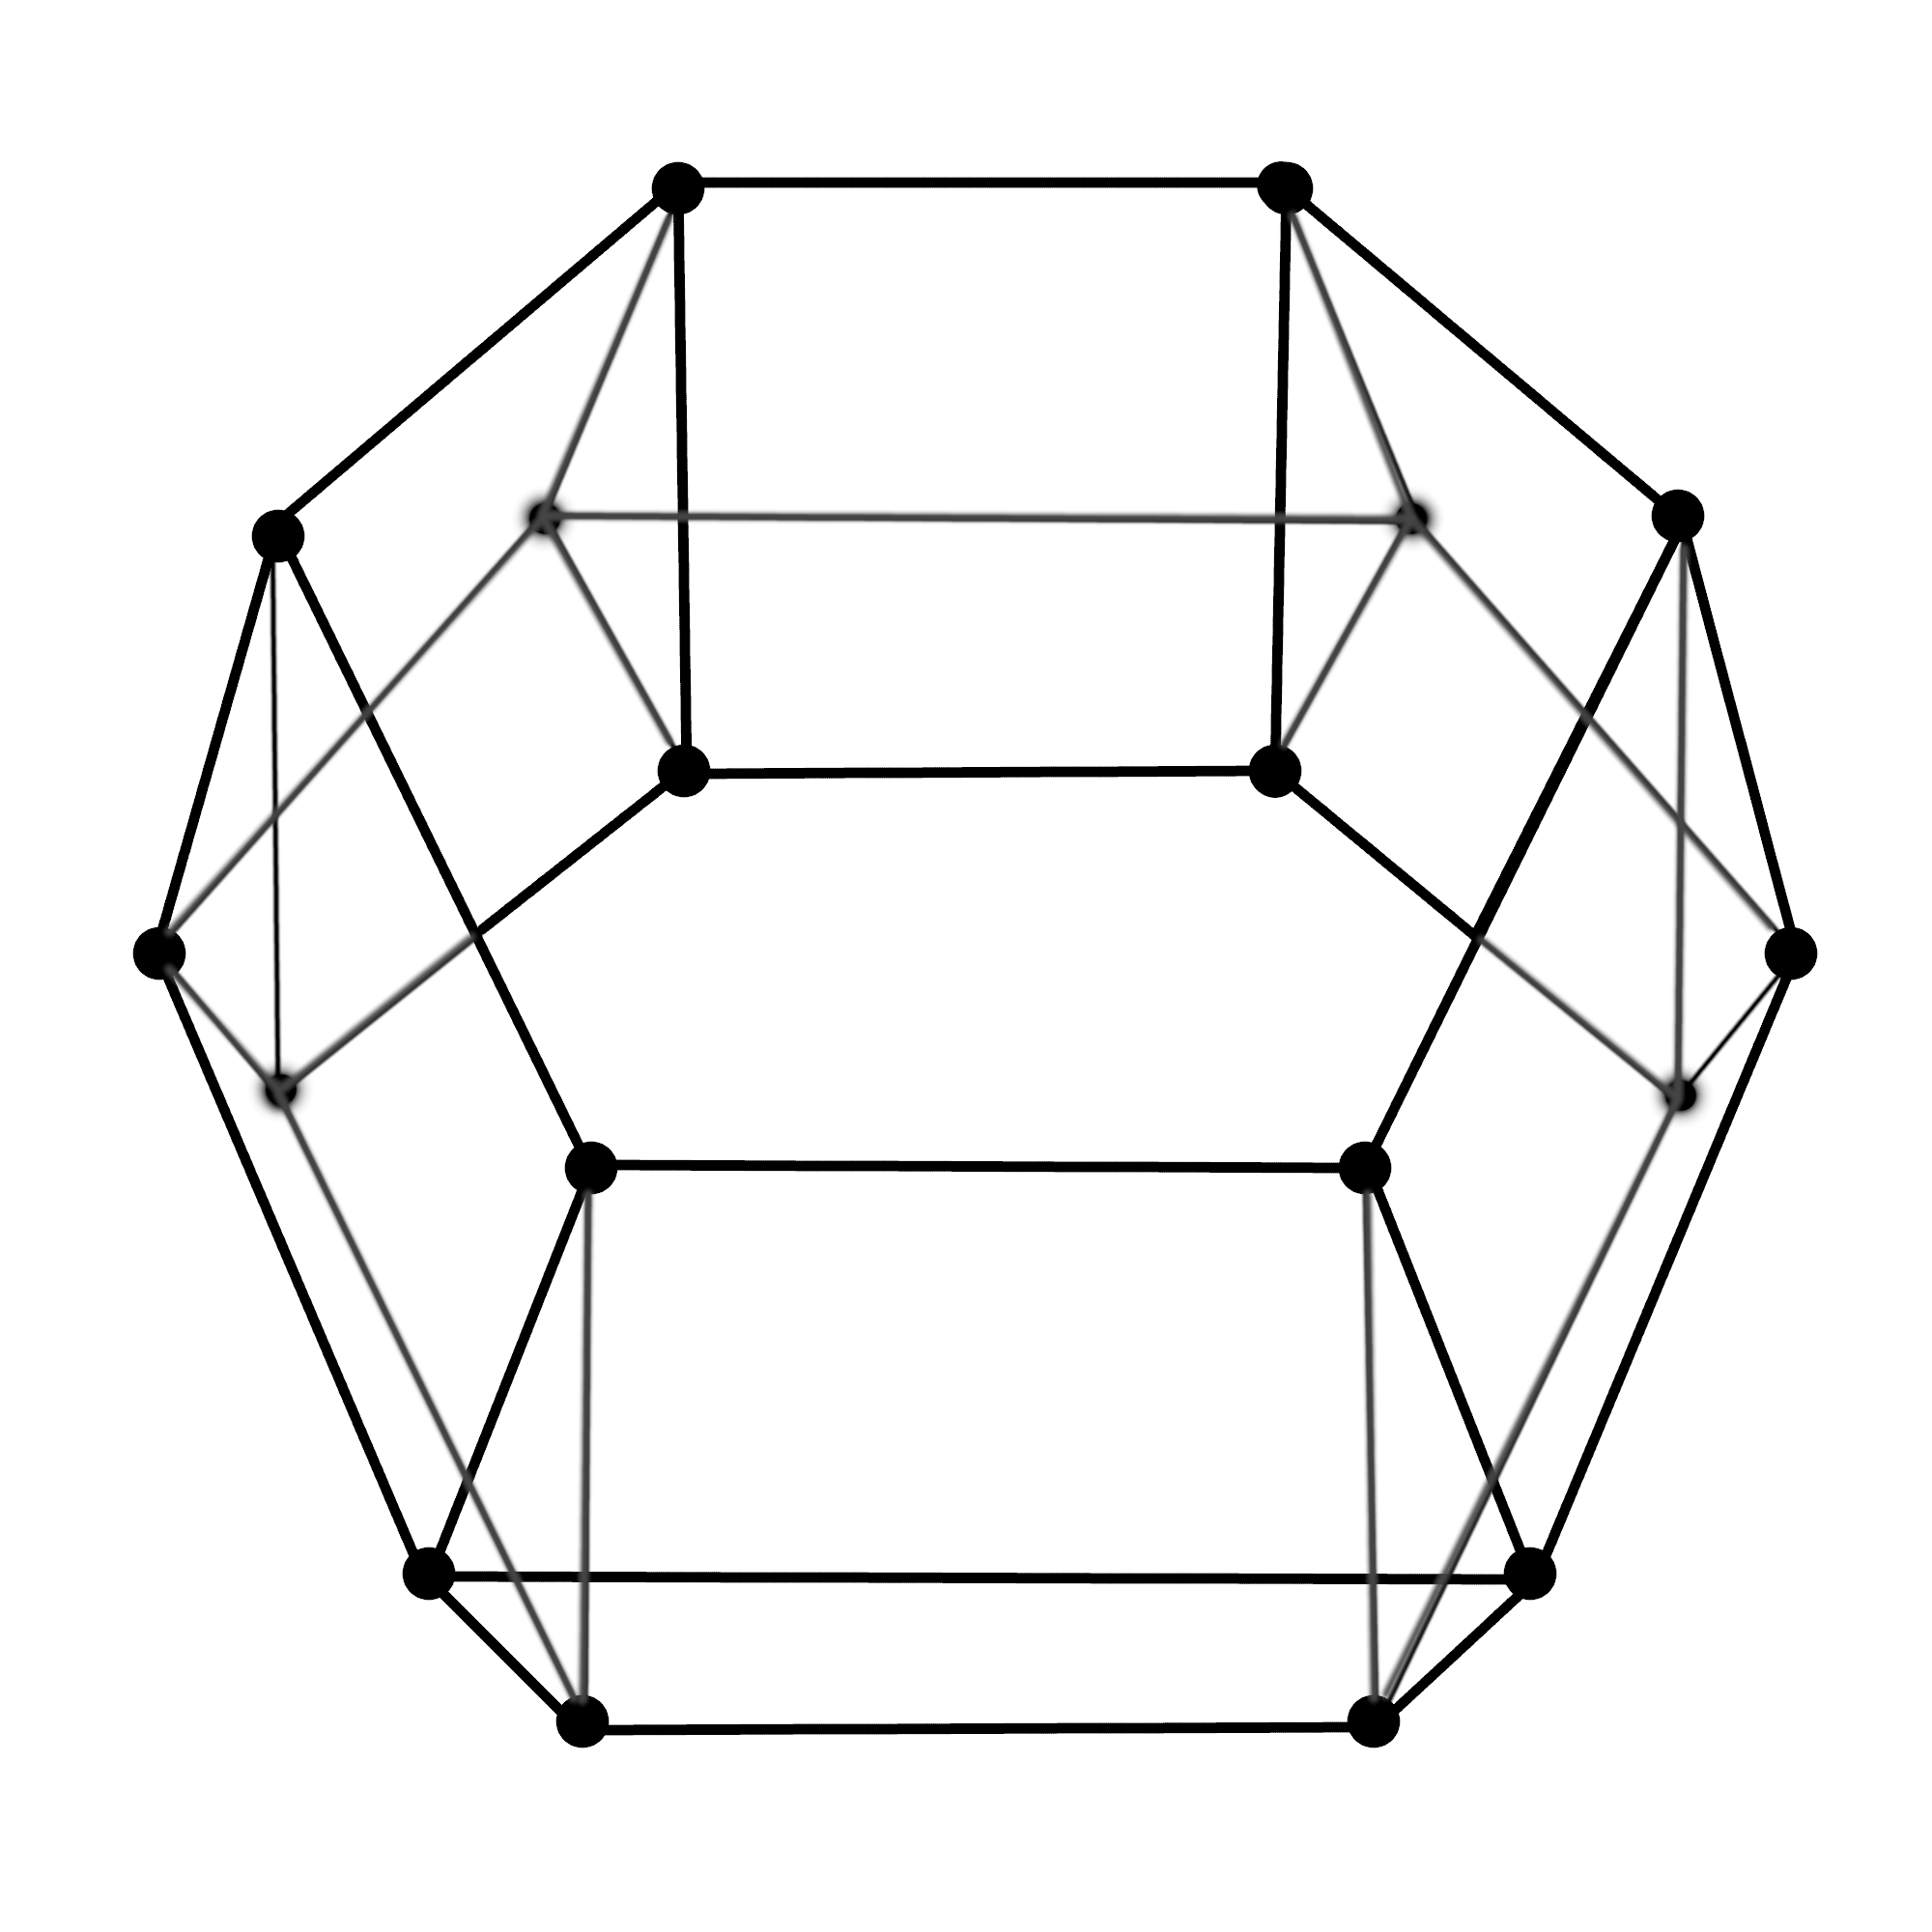
\includegraphics[width=0.25\textwidth]{C3xC6_4.png}
 \caption{$T_{3,6}$}
 \label{c3xc6} %caption vor label unbedingt
\end{figure}
Da wir die Eigenwerte der Laplacematrix eines Kreis-Graphen im Kapitel Warm-up in Gleichung \ref{ewc} schon berechnet haben können wir einfach Satz \ref{tmcpG} anwenden und erhalten
\begin{equation}
 \mathit{k}(T_{m,n})= \frac{1}{mn} \prod_{j=1}^{n-1} 4\sin^2\left(\frac{\pi j}{n} \right)\prod_{i=1}^{n-1} 4\sin^2\left(\frac{\pi i}{n}\right)\prod_{i=1}^{n-1}\prod_{j=1}^{n-1} 4\left(\sin^2\left(\frac{\pi j}{n}\right)+ \sin^2\left(\frac{\pi i}{n}\right)\right)\
\end{equation}
Mit Gleichung \ref{fiktor} können wir schließen
\begin{equation}
 \mathit{k}(T_{m,n})= mn4^{(n-1)(m-1)}\prod_{i=1}^{n-1}\prod_{j=1}^{n-1} \left(\sin^2\left(\frac{\pi j}{n}\right)+ \sin^2\left(\frac{\pi i}{n}\right)\right)\
\end{equation}
\begin{Bsps}[kartesisches Produkt von vollständigen Graphen]
%z.B. rooks graph
\end{Bsps}
Unser Drittes und letztes Beispiel in diesem Kapitel sind kartesische Produkte von vollständigen Graphen. Zu dieser Klasse gehört der Graph, der die legalen Züge des Turms (engl. "rook") auf dem Schachbrett modelliert (siehe Abb. \ref{rook}). Die Graphen dieser Klasse werden daher im Englischen auch als "Rook Graph" bezeichnet.
\begin{figure}[H]
  \centering
 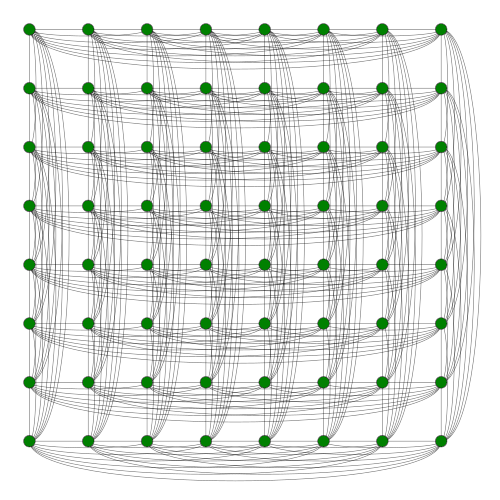
\includegraphics[width=0.5\textwidth]{Rook's_graph.png}
 \caption{Rooks-Graph $\,K_8\times K_8\,$ \\ \tiny{Quelle: \protect\url{https://commons.wikimedia.org/wiki/File:Rook\%27s_graph.svg}}}
 \label{rook} %caption vor label unbedingt
\end{figure}
Um das zu zeigen, berechnen wir zunächst die Eigenwerte der Laplacematrix von vollständigen Graphen und wenden dann Satz \ref{tmcpG} an.
Für $\,n \in \mathbb{N}\,$ ist
\begin{equation}
L(K_n)=
\begin{pmatrix}
n-1&-1&\ldots&\ldots&\ldots&-1\\
-1&n-1&-1&\ldots&\ldots&-1\\
-1&-1&n-1&-1&\ldots&-1\\
\ldots&\ldots&\ldots&\ldots&\ldots&\ldots&\\
-1&\ldots&\ldots&\ldots&-1&n-1\\
\end{pmatrix}
\end{equation}
Wir beobachten, dass das eine zirkuläre Matrix ist, also ist $\,K_n\,$ ein zirkulärer Graph;
Die Eigenwerte kennen wir also schon aus dem enstprechenden Kapitel. Wir setzen die entsprechenden Einträge von $\,L(K_n)\,$ in \ref{cGE} ein und erhalten $\,\lambda_0=0$,\; sowie
\begin{equation}
\begin{split}
 \lambda_j = {} & (n-1) - \sum_{k=2}^{n}\mathrm{exp}{\left(\frac{2\pi \mathrm{i}j(k-1)}{n}\right)}\\
 ={} & n - \sum_{k=0}^{n-1}\mathrm{exp}{\left(\frac{2\pi \mathrm{i}j(k)}{n}\right)}\\
 ={} & n - \left( \frac{1-\mathrm{exp}{\left(\frac{2\pi \mathrm{i}j((n-1)+1)}{n}\right)}}{1-\mathrm{exp}{\left(\frac{2\pi \mathrm{i}j}{n}\right)}} \right)\\
 ={}&n
 \end{split}
\end{equation}
für $\,j\in\{1,\ldots,n-1\}$,\; wobei wir die geometrische Summe verwendet haben; das durften wir, weil hier $\,\mathrm{exp}{\left(\frac{2\pi \mathrm{i}j}{n}\right)} \neq 1\,$ ist.\\
Somit sind die Eigenwerte von $\,L(K_n)\,$ $\,0\,$ mit Multiplizität $\,1\,$ und $\,n\,$ mit Multiplizität $\,n-1$.\; \\
Sei nun $\,m\in\mathbb{N}$.\; 
Für das kartesische Produkt $\,K_m\times K_n\,$ gilt nun mit Satz \ref{tmcpG}
\begin{equation}
 \begin{split}
  \mathit{k}(K_m\times K_n)={}&\frac{1}{nm}(m+0)^{m-1}(n+0)^{n-1}(m+n)^{(m-1)(n-1)}
 \end{split}
\end{equation}

\todo[inline]{vielleicht ein bisschen mehr zu den Beispielen schreiben}
